%%%%%%%%%%%%%%%%%%%%%%%%%%%%%%%%%%%%%%%%%%%%%
%IB pdf source code written by bear blinschauer
%using Stylish article template 

% http://www.LaTeXTemplates.com
% License:
% CC BY-NC-SA 3.0 (http://creativecommons.org/licenses/by-nc-sa/3.0/)

%this project itself wont have a lisence because it will never
%see the light of day after grading and is not profitable
%%%%%%%%%%%%%%%%%%%%%%%%%%%%%%%%%%%%%%%%%%%%%


%----------------------------------------------------------------------------------------
%	PACKAGES AND OTHER DOCUMENT CONFIGURATIONS
%----------------------------------------------------------------------------------------
% {\setlength{\parindent}{0pt}
% \begin{math}
% \end{math}
% }

\documentclass[fleqn,10pt]{SelfArx} % Document font size and equations flushed left

\usepackage[english]{babel} % Specify a different language here - english by default
\usepackage {graphicx, animate}
\usepackage{csquotes}
\usepackage[style=apa,backend=biber]{biblatex}
\addbibresource{MathIA.bib}

\usepackage{xcolor} % Required for specifying custom colours

%----------------------------------------------------------------------------------------
%	COLUMNS
%----------------------------------------------------------------------------------------

\setlength{\columnsep}{0.55cm} % Distance between the two columns of text
\setlength{\fboxrule}{0.75pt} % Width of the border around the abstract

%----------------------------------------------------------------------------------------
%	COLORS
%----------------------------------------------------------------------------------------

\definecolor{color1}{RGB}{0,0,90} % Color of the article title and sections
\definecolor{color2}{RGB}{0,20,20} % Color of the boxes behind the abstract and headings
\definecolor{grey}{rgb}{0.9,0.9,0.9} % Colour of the box surrounding the title

%----------------------------------------------------------------------------------------
%	HYPERLINKS
%----------------------------------------------------------------------------------------

\usepackage{hyperref} % Required for hyperlinks

\hypersetup{
	hidelinks,
	colorlinks,
	breaklinks=true,
	urlcolor=color2,
	citecolor=color1,
	linkcolor=color1,
	bookmarksopen=false,
	pdftitle={Title},
	pdfauthor={Author},
}

%----------------------------------------------------------------------------------------
%	ARTICLE INFORMATION
%----------------------------------------------------------------------------------------

\JournalInfo{Published 2024} % Journal information
\Archive{} % Additional notes (e.g. copyright, DOI, review/research article)

\PaperTitle{Rotation Using Matrix Math} % Article title

\Authors{Name placeholder} % Authors

\Keywords{} % Keywords - if you don't want any simply remove all the text between the curly brackets
\newcommand{\keywordname}{Keywords} % Defines the keywords heading name

\setlength\parindent{24pt}

%----------------------------------------------------------------------------------------
%	ABSTRACT
%----------------------------------------------------------------------------------------

% \Abstract{abstract goes here.}

%----------------------------------------------------------------------------------------

\begin{document}

\begin{titlepage} % Suppresses displaying the page number on the title page and the subsequent page counts as page 1
	%------------------------------------------------
	%	Grey title box
	%------------------------------------------------
\colorbox{grey}{
	\parbox[t]{0.93\textwidth}{ % Outer full width box
		\parbox[t]{0.91\textwidth}{ % Inner box for inner right text margin
			\raggedleft % Right align the text
			\fontsize{20pt}{30pt}\selectfont % Title font size, the first argument is the font size and the second is the line spacing, adjust depending on title length
			\vspace{0.7cm} % Space between the start of the title and the top of the grey box
			\color{color1}\sffamily\bfseries
			IB Analysis and Approaches\\
			Math Internal Assesment\\
			Year Two\\
			\vspace{0.7cm} % Space between the end of the title and the bottom of the grey box
		}
	}
}
	\vspace{-0.5\baselineskip} % Adjust the vertical space between the grey box and the image
	% \begin{figure*}[ht] % Using \begin{figure*} makes the figure take up the entire width of the page
		\raggedleft % Right align the text
		
\includegraphics[width=0.95\textwidth]{cubesTessalation.jpg}
	% 	\label{fig:view}
	% \end{figure*s
	\vfill % Space between the title box and author information
	%------------------------------------------------
	%	Author name and information
	%------------------------------------------------
	\parbox[t]{0.93\textwidth}{ % Box to inset this section slightly
		\raggedleft % Right align the text
		\large % Increase the font size
		{\Large Name Placeholder}\\[4pt] % Extra space after name
		Analysis and Approaches student\\
		Roosevelt High 2024\\[4pt] % Extra space before URL
		\hfill\rule{0.2\linewidth}{1pt}% Horizontal line, first argument width, second thickness
	}
\end{titlepage}

\maketitle % Output the title and abstract box

\tableofcontents % Output the contents section

\thispagestyle{empty} % Removes page numbering from the first page

%----------------------------------------------------------------------------------------
%	ARTICLE CONTENTS
%----------------------------------------------------------------------------------------
\section*{Introduction}

\addcontentsline{toc}{section}{Introduction} % Adds this section to the table of contents

\hspace{\parindent}%tab
As an individual, I am fascinated by 3d graphics and research the topic on my own time. Mathematical applications in computer graphics is a fascinating part of both computer science and math. The idea that math is able to describe entire virtual environments is remarkable. Among other important mathematical concepts, vectors and rotational transformations play a crucial role in the positioning of objects in three-dimensional spaces.

%Often while trying to learn 3d graphics I get roadblocked by rotation vectors and the trigonometry inside the function appears intimidating.
Although there are alternative systems of rotation that avoid problems such as Gimbal Lock, in this math Internal Assessment I decided to use rotation matrices and learn how they work using the unit circle. I decided to focus on rotation matrices because they allow us to use Euler angles and build up important knowledge of linear algebra. Knowing how these systems work is important because it allows the individual to make an end product more intuitively and to work in 3d space without any help or helper libraries.

This assessment will connect to trigonometry. I will utilize basic trigonometry to reason vector composition, and I will use the unit circle in order to visualize vector rotation. In order to break down the task, I will divide the problem into smaller, more manageable problems that build on each other. Not only will I explain the math behind these methods of rotation, but I will also use math I already know to implement the rotational algorithms in C++ and JavaScript on my own. During this project, I will be writing multiple visualization programs, making GIF's 
\footnote{Note on animations: gifs are represented as image urls pointing to an animated gif, this is because free pdf viewers like firefox dont support most pdf animations and scripting. IB auditors may be disalowed from resolving image get requests due to software limitations. In this case a description will be added in the margins.}
 that demonstrate the math I learn.  The final project that I will produce will be a simple program rotating a triangle in 3d space.

\section{Problem}
% \addcontentsline{toc}{section}{Problem} % Adds this section to the table of contents

\hspace{\parindent}%tab
The problem for the math internal assessment is as follows. I need to derive a method to create rotations in three-dimensional space by using trigonometry and basic linear algebra.

This problem is very important to everyday life powering many aspects of video games, CAD, and complex milling. The problem with rotation has an elegant system of solutions that builds up to more complicated and important problems.

Trigonometry (the study of angles) is integral in the rotation process. In rotation matrices, trigonometric functions are used in order to calculate rotation and position. Trigonometry is also utilized to more generally in linear algebra in order to calculate the angle and position of resultant vectors, which is integral to the process.

\section{Math}

\hspace{\parindent}%tab
% Coming to a conclusion on how to represent a three dimensional rotation using triginometry is a complex task so 
In order to make the layout of this document easier to understand the math section will be broken into smaller chunks of a larger recipe. Eventually we will make a working demo in open Gl or three.js, but before we compute beautiful rotations I will have to clear the air on the math behind the magic and the process I used to find it first.

% \paragraph*{Parts:}
% \begin{enumerate}[noitemsep] % [noitemsep] removes whitespace between the items for a compact look
% 	\item Defining 2d transformation
% 	\item Apply trigonometry in order to transform things rotationally.
% 	\item Applying rotation in 3d
% 	\item Multiplying matrices in 2d and then 3d in order to get combined pitch yaw roll rotations on new axis.
% 	\item Implementing 3d rotation on objects using a graphics library.
% \end{enumerate}

\subsection{Defining 2d Transformation}
\hspace{\parindent}%tab
In order to understand 3d rotation It would be much simpler to start with simpler problems such as transforming objects in 2d space. Part one will explore how to actually get 2d vectors to move.

To start making vectors move, we should first define what a vector is. Different areas of math define vectors differently, such as physics, who define vectors as a scalar with an angle attached to it. In a mathematical point of view, a vector can be represented in a diversity of formats. Since matrix operations will be performed on the vector in this context the vector is defined as a matrix that defines coordinates in space pointing away from the origin. Essentially, this vector is a matrix that contains two perpendicular vectors that add up to the final vector.

\begin{equation} \vec{v} = \begin{bmatrix} x \\ y \end{bmatrix} \end{equation}

% \begin{math}
% 	\vec{v}=\begin{bmatrix} x \\ y \end{bmatrix}
% \end{math}

In order to construct the vector from the two coordinates, we can use trigonometry to find the angle of the vector and the Pythagorean theorem to find its magnitude.

\begin{align} \theta &= \arctan\left(\frac{y}{x}\right) & \lvert \vec{v} \rvert = \sqrt{x^2 + y^2} \end{align}

In order to add two vectors together, the resulting vector is the x components added together and the y components added together. By adding two vectors and multiplying either by a scalar, the base vectors will be able to represent any other vector in 2d space as long as they don’t have the same angle. These two vectors would represent the axis of the resulting vector. We say that these two vectors have a range of all two-dimensional space.
\begin{align}\label{eq2}
	\vec{s}&=\left[\begin{array}{llllllllll}x_1+x_2 \\y_1+y_2\end{array}\right] &
	\vec{v}=x*\vec{i}+y*\vec{j}
\end{align}

The basis vectors are denoted by i and j. Any vector can be represented as a combination of these. By default, the basis vectors on the xy plane are simply scaled as one to make math more sensible. i and j are perpendicular and not rotated because the coordinates on a graph are typically vertical and horizontal.

\begin{equation}
	\overset{\wedge}{i}=\begin{bmatrix} 1\\0 \end{bmatrix} \overset{\wedge}{j}=\begin{bmatrix} 0\\1 \end{bmatrix}
\end{equation}


The basis vectors give us one of the fundamental ideas in transformation linear algebra where any vector can be written as two scalars scaling two basis vectors. Basis vectors are similar to the unit circle in trigonometry. If the coordinates of the basis vectors change, the resulting plane of 2d space the basis vectors represent will also change. 

What we have learned is revolutionary, in order to change any set of vectors we can instead change the coordinates of the basis vectors and then apply the new basis vectors to all vectors we want to change. In order to denote a transformation like this, we can represent the transformation as a matrix represented by t. Here, the matrix is made up of vectors i and j. In order to apply the transformation, we multiply the transformation matrix by the vector we want to transform. 
\begin{equation}T=\begin{bmatrix} i_{x} & j_{x} \\ i_{y} & j_{y} \end{bmatrix}\end{equation}
In this way we can apply intuition in order to define a simple algorithm of multiplying a matrix by a vector.
\begin{equation}\begin{bmatrix} a & b \\ c & d \end{bmatrix}\begin{bmatrix} x \\ y \end{bmatrix} = x\begin{bmatrix}  a \\ c \end{bmatrix} + y\begin{bmatrix} b \\ d \end{bmatrix} = \begin{bmatrix} ax+by \\ cx+dy \end{bmatrix}\end{equation}
% Note above equation is essentially equation \ref{eq2} but represented as matrices instead of letters with arrows on top of them. Knowing how to transform 2d vectors like this is really useful and the same transformations can be adapted for 3d space.

\subsection{Triginometry and Rotation}
\hspace{\parindent}%tab
Simply scaling the basis vectors allows the user to scale and shear, which is really useful but not our ultimate goal. In order to rotate the vectors, we will need to rotate the axis using the unit circle. The unit circle is represented as a circle with radius one. In order to calculate trigonometry values, a point along the unit circle is used. This point consists of two numbers less than one. In the unit circle, the x coordinate of the point is the cosine and the y coordinate is the sine. Together, the sine and cosine coordinate represent a normalized vector of length one. These types of vectors are called unit vectors and solely represent an angle.

\begin{figure}[ht]\centering % Using \begin{figure*} makes the figure take up the entire width of the page
	\includegraphics[width=\columnwidth]{images/unitCircle.png}
	\caption{The Unit Vector}
	\label{fig:unitVec}
\end{figure}

By using our knowledge about the relevance of unit circles, it is simple to assume that one can simply scale the basis vectors by sine and cosine. Astute mathematicians will start to notice flaws in this plan. For example the magnitude of rotated vector $\vec{v}=\begin{bmatrix}1\\1\end{bmatrix}$ will not preserve its magnitude and will have a magnitude of 1 instead of $\sqrt{2}$. With further investigation, this approach doesn't work. Some transformation similar to rotation is gained, but the magnitude is not preserved. When transforming images, it is apparent the unintended stretching of the x-axis and y-axis causes the image to appear distorted. In order to visualize the transformations in in effect animations were made below.


\begin{figure}[ht]\centering % Using \begin{figure*} makes the figure take up the entire width of the page
\begin{tabular}{ c c }
	\href{https://raw.githubusercontent.com/beastr45/MathIA-bear/main/latex/Figures/images/gifs/VectorT1.gif}{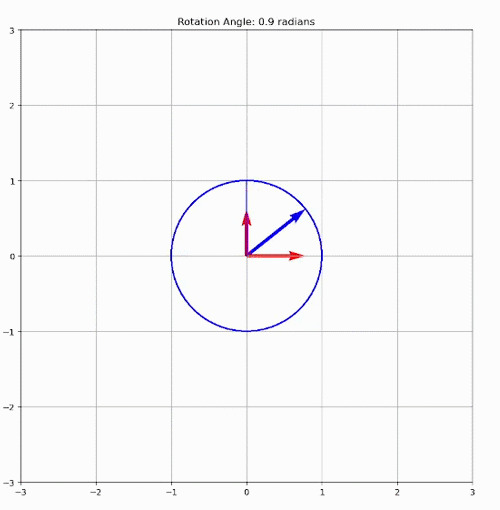
\includegraphics[width=\columnwidth/4]{images/VectorT1-24.jpg}} & \href{https://raw.githubusercontent.com/beastr45/MathIA-bear/main/latex/Figures/images/gifs/VectorT1Fail.gif}{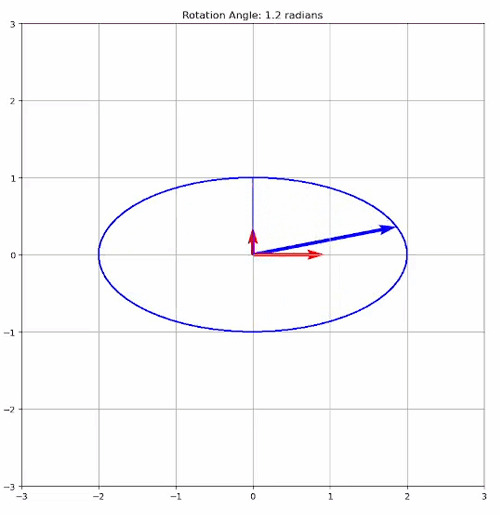
\includegraphics[width=\columnwidth/4]{images/VectorT1Fail-30.jpg}}
 % cell1 & cell2 \\
 % cell4 & cell5 \\
\end{tabular}
	\caption{With symmetrical vectors rotation appears normal but with vectors where y dosent equal x it is apparent stretching occurs.}
	\label{fig:exGifs}
\end{figure}

In order to transform a vector, we will instead take the unit vectors themselves rotate them across the unit circle. In order to do this we can apply the same type of transformation that we tried earlier to the base vectors instead of the resulting vector. We are now essentially making two transformations, one transforming all the basis vectors by theta and the other multiplying the rotated basis vectors with the vector we want to transform. This system prevents a change in magnitude of the vector that we want to transform.

\begin{figure}[ht]\centering % Using \begin{figure*} makes the figure take up the entire width of the page
\begin{tabular}{ c c }
	\href{https://raw.githubusercontent.com/beastr45/MathIA-bear/main/latex/Figures/images/gifs/rotFailMonkey.gif}{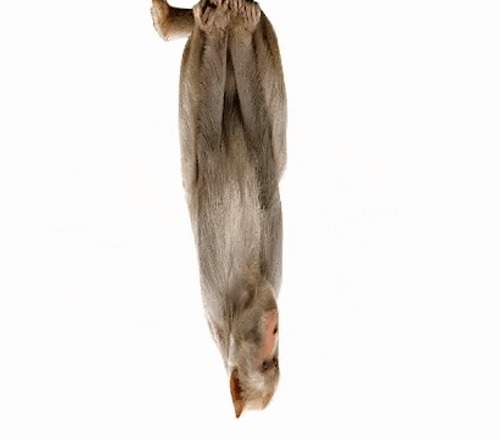
\includegraphics[width=\columnwidth/4]{images/rotFailMonkey-33.jpg}} & \href{https://raw.githubusercontent.com/beastr45/MathIA-bear/main/latex/Figures/images/gifs/monkeyRotation.gif}{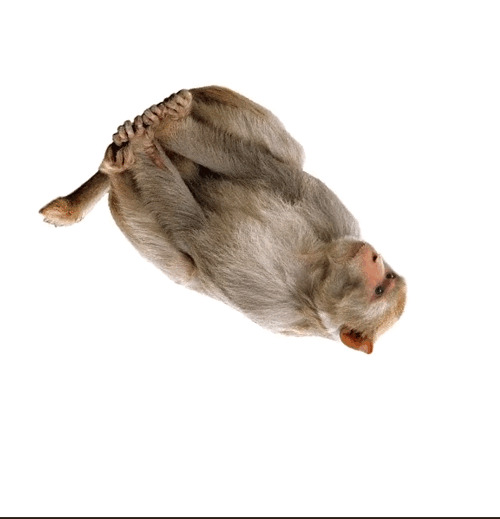
\includegraphics[width=\columnwidth/4]{images/monkeyRotation-78.jpg}}
 % cell1 & cell2 \\
 % cell4 & cell5 \\
\end{tabular}
	\caption{With a monkey refrence it is clear of the benefits of an absence of stretching/shearing}
	\label{fig:monkeyGif}
\end{figure}

In order to transform a basis vector by theta we set the components of the basis vector to be sine and cosine. Since j is on the y-axis sine and cosine are flipped with sine being negative. This is simply due to the fact that the initial orientation of the transformation is itself 90 degrees from the x-axis. This process is visualized below. 

\begin{figure}[ht]\centering % Using \begin{figure*} makes the figure take up the entire width of the page
	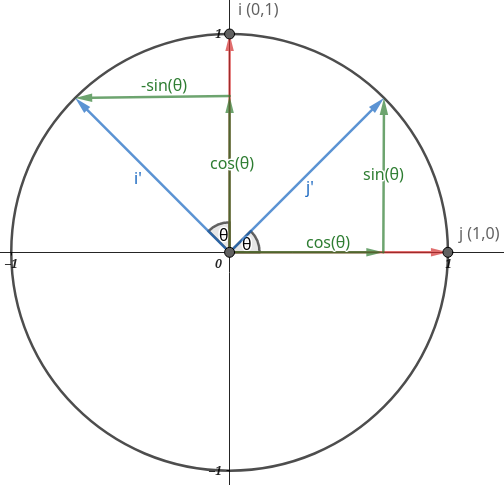
\includegraphics[width=\columnwidth]{images/GeogebraVis.png}
	\caption{The effect of the transformations on the basis vectors is illustrated.}
	\label{fig:TransformationDiagram}
\end{figure}

by using the coordinates of i and j the rotation matrix can be defined as follows

\begin{equation}
	\begin{bmatrix} \cos{\theta} & -\sin{\theta} \\ \sin{\theta} & \cos{\theta} \end{bmatrix}\begin{bmatrix} x \\ y \end{bmatrix} = \vec{v^{\prime}}
\end{equation}

\subsection{3d Rotation}
\hspace{\parindent}%tab
Now that we have a better way to represent 3d rotation, we can apply it to 3d. The same idea that transformation matrices is a collection of basis vectors still works in the third dimension. 

In 3d space, when we want to rotate things with rotation matrices, we can only rotate in one direction at a time. So in our rotation matrix, we can avoid the axis that is being rotated around and treat the problem the same way as 2d rotation. In the rotation matrix you can see the basis vector in the axis of rotation is not affected and the components of the basis vectors that do transform ignore change in that same axis.

\begin{figure}[ht]\centering % Using \begin{figure*} makes the figure take up the entire width of the page
	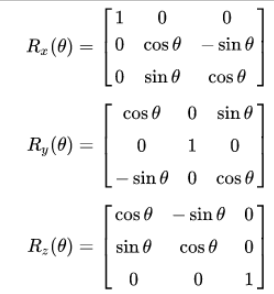
\includegraphics[height=\columnwidth/2]{images/matrixRef.png}
	\caption{3-dimensional rotation matrices}
	\label{fig:3dTransformationDiagram}
\end{figure}

In order to get a more complex rotation, the rotation matrices x y and z can be multiplied together. When multiplying matrices the order matters, a rotation over y-axis and z axis will produce a different vector than a rotation in the z axis and then y-axis. It is also important to note that rotating in three axis will result in unpredictable behavior when the rotation axis line up. This is called gimbal lock.

\subsection{Graphics Implementation}
\hspace{\parindent}%tab
The most important part of the math IA is the implementation of rotation algorithms into real world application because it demonstrates that the IB student is capable in their understanding of the topic. The implementation shows the student did math and gives meaning to the internal assessment instead of having it be conductive of meaningless research. In this math Internal Assessment rotations have a very practical and tangible use in computer graphics. 

Rotation matrices are used in computer graphics in order to calculate movement and shading. Initially an variety of ideas were proposed in order to demonstrate the topic. Lots of mediums can be used to transform 3d objects such as Desmos or Open Gl but more complex implementations were cut due to complexity and lack of time. To get started implementing rotation matrices the three.js library is used in order to render the required images.

3d files contain a series of vectors connected together. In order to render a 3d file we can just put the x and y coordinates on a plane excluding the z coordinates. In order to remove the z coordinates a system called projection scales vectors farther away of the z axis giving the illusion of depth. In this case three.js takes care of this.

\begin{figure}[ht]\centering % Using \begin{figure*} makes the figure take up the entire width of the page
	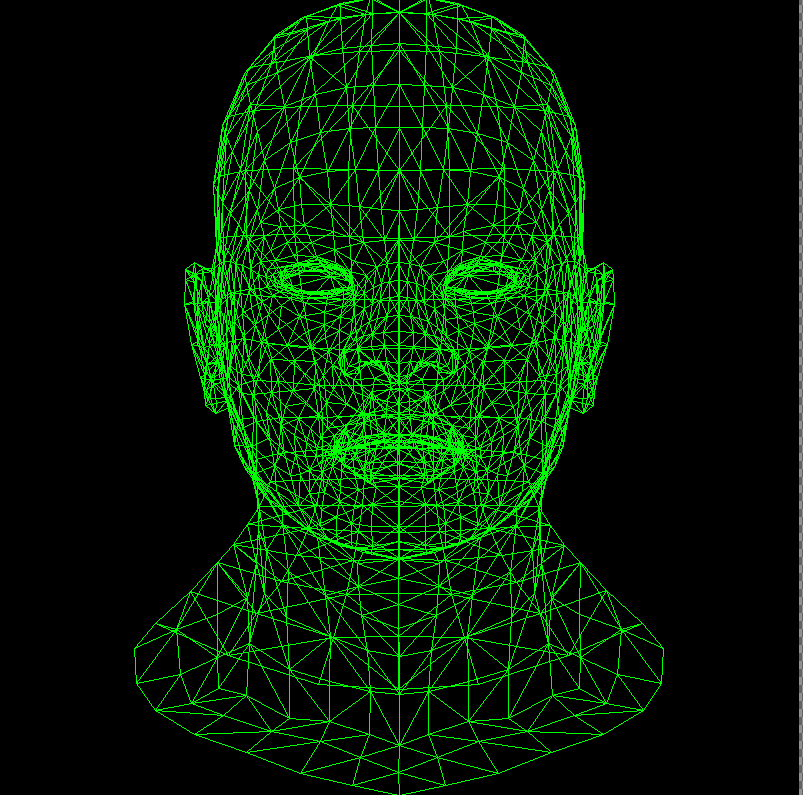
\includegraphics[width=\columnwidth/2]{images/TinyrenderSkull.png}
	\caption{Tiny render demo: Isometric model rendered excluding depth}
	\label{fig:wireframe}
\end{figure}

This works well but in order to rotate an object we will need to perform a rotation to each of the vertices before the redundant axis is removed. In order to do this in the code our computer will make matrix transformations on each vector in the 3d file and then project it onto our screen.

In order to simulate three-dimensional rotation a program was written in order to apply the rotation matrices to every vertex in a 3d file, demonstrating in practice how rotation matrices would be utilized in the industry.
\begin{figure}[ht]\centering % Using \begin{figure*} makes the figure take up the entire width of the page
\begin{tabular}{ p{0.45\columnwidth} p{0.45\columnwidth} }
	\href{https://raw.githubusercontent.com/beastr45/MathIA-bear/main/latex/Figures/images/gifs/humanRotate.gif}{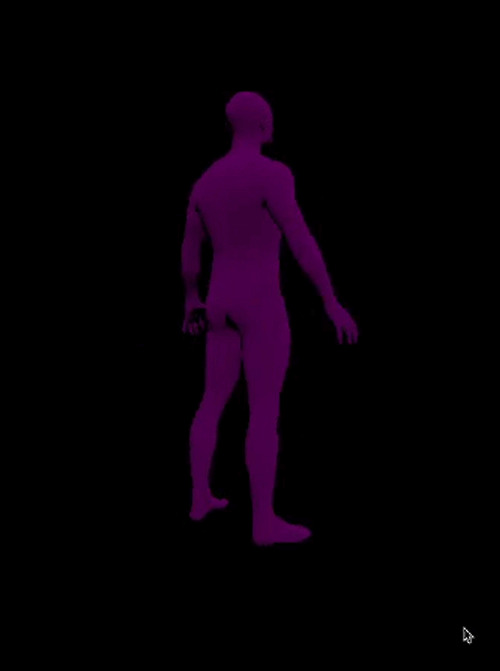
\includegraphics[width=\columnwidth/3]{images/humanRotate-38.jpg}} & \href{https://raw.githubusercontent.com/beastr45/MathIA-bear/main/latex/Figures/images/gifs/humanRotate.gif}{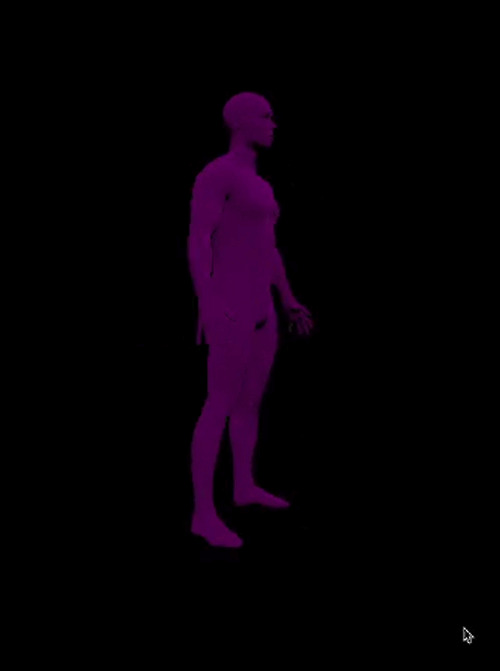
\includegraphics[width=\columnwidth/3]{images/humanRotate-46.jpg}}
 % cell1 & cell2 \\
 % cell4 & cell5 \\
\end{tabular}
	\caption{Demo of a model rotating using matrix math.}
	\label{fig:humanGif}
\end{figure}
\section{Conclusion}
\hspace{\parindent}%tab
In while rotation matrices initially appear complex, the trigonometry behind it connects heavily to the unit circle we learned about in class. Knowing the fundamental math ideas behind transformations gives us the tools in order to construct a better mathematical system to interact with 3d and 2d space. Rotational transformations are not just useful for their academic benefit and form a great deal of importance due to their relevance in computer graphics. 
\section{Reflection}
\hspace{\parindent}%tab
Even though 3d math is really complicated, it is also very fascinating to learn about. This math IA is part of a larger project of mine where I try to build a 3d renderer from scratch. Although I haven't really thought too far into my extended essay. I think that as an extension to the topic I might make this IA part of my larger extended essay. 

It's a bummer I didn’t get to focus more on the actual computer science implementation of rotation very much because the implementation was the step I was most excited for while choosing my math IA. Overall I just didn’t have enough time and the other parts of the graphics pipeline I would have to implement first would make the project super complex. It is better that I didn’t focus my math IA less ma-thy things because although fascinating to a mathematician It would most likely not make very much sense to the reader.

% {\setlength{\parindent}{0pt}
% \begin{math}
% 	 \theta = \arctan\left(\frac{y}{x}\right)
% \end{math}
% }
% \vspace{10pt}%tab
% {\setlength{\parindent}{0pt}
% \begin{math}
% 	 \lvert \vec{v} \rvert = \sqrt{x^2+y^2}
% \end{math}
% }
% \href{http://www.google.de}{\includegraphics[width=\linewidth]{ unitCircle.png}}
% \includegraphics[width=\linewidth]{images/unitCircle.png}
%adobe sucks just give up and link to raw github content
% \animategraphics[scale=0.4,loop,autoplay]{30}{Figures/monkeyRotation/foo-}{0}{99}
% \noindent\animategraphics[scale=0.9,controls,step]{0}{animate}{}{}



%----------------------------------------------------------------------------------------
%	REFERENCE LIST
%----------------------------------------------------------------------------------------
\phantomsection
\nocite{*}
\begin{flushleft}
  \printbibliography
\end{flushleft}
% \printbibliography
% \bibliographystyle{unsrt}
% \bibliography{MathIA.bib}
%
\textcolor{red}{41 75 74 68 6F 72 3A 20 42 65 61 72 20 42 6C 69 6E 53 63 68 61 75 65 72}

%----------------------------------------------------------------------------------------

\end{document}
